
\chapter{Numerical Model Fitting}
\label{chapter4}

With the ability to generate an equilibrium solution for the GSH equation from chapter \ref{chapter3}, 
our next goal is to be able 
\todo
In chapter \ref{chapter3} we developed the ability 

% 4.1.
\section{Non-Linear Optimisation}

Optimisation methods are, at their heart, minimisation problems (and dually maximisation problems, 
though the two are equivalent). We have some function $f(x)$, called the \textit{objective function},
and some domain $\Omega \subset \R^n$, and we wish to determine
$$\arg\min_{x \in \Omega} f(x)$$
Often the objective function is accompanied by a set of constraints, which more or 
less are used to define the set $\Omega$. If we let $c_i(x) \ge 0$ describe one of $k$ constraints that $f$ 
is subject to, then we can describe $\Omega$ as such:
$$\Omega := \lbrace x \in \R^n : c_1(x) \ge 0 \; \land c_2(x) \ge 0 \land \dots \land c_k(x) \ge 0 \rbrace$$

\begin{remark}
    If a given problem has no constraints (i.e. you are only presented with the task of minimising a function), then 
    this is known as an \textbf{unconstrained optimisation} problem. As soon as you add constraints however, you have a 
    \textbf{constrained optimisation} problem. Algorithms may have better or worse performance in reaching a local minimum 
    depending whether the problem is constrained or not.
\end{remark}

There are a number of difficulties that come packaged with optimisation problems. Firstly, 
the method by which you go about minimising your function is dependent on the properties of your function 
- you will have a much easier time minimising a smooth, convex function than you would a discontinuous, 
non-convex function, and different algorithms will net you varying results for each. Another factor 
that affects the choice of optimisation methods available, is the linearity of your system. Often linear systems 
can have ``nice'' methods of solving them. However, the behaviour of non-linear systems can often make them 
unwieldy when it comes to finding local and/or global minima. 

\begin{definition}[Non-linear Optimisation Problem]
    Let $x \in \Omega \subseteq \R^n$. Also let $f:\Omega \to \R$ be the objective function, and $c_i :\Omega \to \R$ and $d_j : \Omega \to \R$ be 
    constraints. Then a non-linear optimisation problem is a problem
    \begin{align*}
        &\min_{x \in \Omega} f(x) \\
        c_i(x) &\ge 0 \;\; \forall i \in \lbrace 1, \dots, m \rbrace \\
        d_j(x) &= 0 \;\; \forall j \in \lbrace 1, \dots, p \rbrace
    \end{align*}
    where one of $f$, $c_i$ and/or $d_j$ are non-linear.
\end{definition}


% 4.1.1.
\subsection{Least Squares}

Least squares problems are a subsect of optimisation problems, which are largely concerned with fitting some function to 
a set of data. Let a set of data be given $(x_i, y_i)$, where $x_i$ are independent variables, and $y_i$ are dependent variables in 
the data set. We wish to fit some function $f(x, \beta)$ to fit our data as tightly as possible, where $x$ is the independent variable 
as for the data, and $\beta$ are parameters in the function $f$ which can be varied. Let $r_i$ be the \textit{residual} error between 
a given data entry $(x_i, y_i)$ and our corresponding value for it, $f(x_i, \beta)$ for a given $\beta$. Then our goal 
(in wanting to have a function $f$ which matches the provided data) is to reduce the amount of residual error we have - to minimise it. 
We can specify this as an optimisation problem \cite{carlone-least-squares}
\begin{align*}
    \min_{\beta \in \Omega} \sum_{i = 1}^{n} \norm{r_i(\beta)}^2 = \min_{\beta \in \Omega} \sum_{i = 1}^{n} \norm{y_i - f(x_i, \beta)}^2
\end{align*}
In this case, our objective function is the equation $g(\beta) = \sum_{i = 1}^{n} \norm{y_i - f(x_i, \beta)}^2$.

\begin{remark}
    While the above norm is left general, often optimisation algorithms will take this to be the $L^2(\R^n)$ norm.
\end{remark}
\begin{remark}
    The above is, by default, an unconstrained optimisation problem. When we come to formulate our own least squares problem, we will 
    introduce our own constraints however. Additionally, the above is not specified to be linear or non-linear. In our efforts, 
    we will deal with a non-linear system.
\end{remark}

Thus, if you are provided with a set of data, and a function you wish to use to approximate the behaviour of the data, you can 
employ the use of a least squares optimisation method to manipulate that function into being as close a fit to that data as 
it can be. How we implement that optimisation is a question of algorithms, which we will now cover.

% 4.1.2.
\subsection{Optimisation Algorithms}

\begin{notn}
    When we talk about running algorithms to solve our optimisation problems, we will use a few terms. We define those here:    
    \begin{table}[h!]
        \begin{tabular}{p{3.5cm}|p{10cm}}
            \textbf{Feasible} & A problem is feasible if the algorithm is able to find an $x^* \in \Omega$ that is a local minimum and satisfies any given conditions. Otherwise, it is \textbf{infeasible}. \\ \hline
            \textbf{Objective Value} & The value of the objective function for the identified local minimum $x^* \in \Omega$, $f(x^*)$ . \\ \hline
            \textbf{ftol} & If the difference between consecutive objective function values is less than this amount, stop the optimisation algorithm and return converged \\ \hline
            \textbf{xtol} & If the difference between consecutive $x \in \Omega$ values is less than this amount, stop the optimisation algorithm and return converged \\ \hline
        \end{tabular}
    \end{table}
    
\end{notn}

The main questions that an optimisation algorithm asks at each of its iterations is: which direction should I travel, and how far 
should I travel in that direction? Algorithms that use this form of logic are called \textit{descent methods}, and a 
general approach for them is given \cite{carlone-least-squares}:

\begin{algorithm}[h!]
    \begin{algorithmic}[1]
        \State Given initial guess $x$
        \While {Convergence criteria not satisfied}
            \State Choose (unit) descent direction $\delta_x \in \R^n$
            \State Choose step size $\gamma \in \R$
            \State $\delta \leftarrow \gamma \cdot \delta_x$
            \State Update variables $x = x + \delta$
        \EndWhile
    \end{algorithmic}
\end{algorithm}
Thus, descent algorithms are distinguished by the mechanism by which they choose a descent direction, and the step size.

While the algorithms we will talk about here can be applied to optimisation problems generally, we should 
keep in mind their application to non-linear least squares problems, as this is what we will eventually deal with. 
Here we'll provide an overview of two common algorithms 
used for finding local minima of a given function. In our attempts to fit a model to some data in section 4.2, we first 
attempted to use these methods. However, due to the nature of the objective function we have, these efforts were in vain, and 
we turned to a different algorithm (MMA). Nevertheless, it is useful for intuition to see examples of other algorithms.

\subsubsection{Newton's method}
Newton's optimisation method exploits a Taylor series expansion of a given objective function. Assume that we 
want to determine $\min f(x)$, where $x,\delta \in \R^n$. We know that an expansion about $x + \delta$ is:
\begin{equation*}
    f(x+\delta) \approx h(x+\delta) := f(x) + \nabla f(x)^{T} \delta + \frac{1}{2}(\delta)^{T} \nabla^2 f(t) \delta
\end{equation*}
where $\nabla^2$ denotes the Hessian. We want to find a turning point (minimum) of the above, so we can simply set its 
derivative to be $0$. This gives us
\begin{equation*}
    \nabla f(x) + \nabla^2 f(x) \delta = 0
\end{equation*}
This tells us that the optimal descent direction (and step size) is
\begin{equation*}
    \delta = - \gamma \left [  (\nabla^2 f(x))^{-1} (\nabla f(x)) \right ]
\end{equation*}
where $0 < \gamma \le 1$ is a chosen step size, which can be tailored to a given problem. 

\begin{remark}
    As Newton's method only necessitates that the objective function be twice differentiable, it is applicable to 
    optimisation problems generally (i.e. it is not restricted to constrained nor unconstrained problems, nor does it differentiate 
    between linear and non-linear problems).
\end{remark}

\subsubsection{Gradient descent}
Gradient descent is an approach which has strong intuitive roots. If you were at the top of a hill, and wanted to get 
to the bottom as fast as possible, then you might choose to go down the steepest point you see around you. This is 
essentially what gradient descent does. For an objective function $f(x)$, assuming that it is differentiable 
for some neighbourhood of a point $a \in \R^n$, then the optimal descent direction is $- \nabla f(a)$. This can, 
similar to Newton's method, be scaled by a step size $\gamma$ to slow / speed up this process, though the value of 
this is dependent on the optimisation problem you're investigating (note that, similar to Newton's method, 
the gradient descent method can be applied to a large class of problems).

\subsubsection{MMA}
One of the problems we encountered in our data fitting attempts (which we will see in the next section), is that 
of asymptotic behaviour which affects convergence of our algorithms. Thus, we sought to employ the use of an algorithm 
which was more resistant to such behaviour in an objective function. This led to the discovery of the Method of Moving 
Asymptotes algorithm, developed 
by Svanberg \cite{mma}. While its implementation details are a bit volumous to repeat here, in essence, it works by creating 
convex sub-problems around potential local minima, and attempts to minimise these individually. It repeats this process until 
it is no longer decreasing, and returns the most recent potential local minima it found. This algorithm is 
useful to us two main reasons: 1. it is still as robust an optimisation method as Newton's method and gradient descent, in that it 
can handle a host of optimisation problems (including non-linear problems); and 2, it is more resistant to the asymptotic behaviour.

In our code we use an implementation provided by the NLopt package, a nonlinear optimisation library for Julia \cite{nlopt}. The NLopt
library, in iniitialising an optimisation problem for MMA, requires information about the objective function, its partial derivatives, 
and any constraints, if they exist (which they will for us, but we'll note on that shortly). Thus, when it comes to constructing 
our system, we must provide the objective function naturally, but also its partial derivatives with respect to our paramters.

% 4.2.
\section{GSH Parameter Fitting}

In the previous chapter we were able to, given $P := (a_1, a_2, \alpha)$, reproduce results from Wang, including 
the poloidal magnetic flux, current density profile, and pressure density profile. However, in reality, we will 
not know these parameters $P$ for a given system - yet we are entirely dependent on them for describing our system. 
We then face a problem, which is that if we wish to vary our system, or if we wish to describe a real tokamak's dynamics,
we need some way to determine what $P$ should represent the system we're investigating. 

Looking forward a bit, we know that from the ISTTOK project we have time series current density profile and pressure density profile data 
available to us. Thus we may wish to utilise at least one of these in determining $P$ - and this is exactly what we will do. 
In the previous section we built the theory for, given a set of data, fitting a function $f$ with variables $\beta$ which can be varied, 
which is exactly the challenge we now face. 

We could seek to use both the current density profile and pressure density profile, and could build an objective function around this. However, 
we will also note that we wish to verify our results - as such, it may be prudent to leave one of these data sets available for comparison instead. 
With a bit of prescient knowledge we may realise that derivatives are much easier to calculate for the current density profile, and so choose 
to build our objective function around this, reserving pressure density data for comparisons instead. In the spirit of laziness, this is 
exactly what we do.

In this chapter we will not concern ourselves with experimental data however - that is the task of chapter \ref{chapter5}. Here we 
will work with contrived data. With our ability to specify parameters $P$ and derive the equilibrium solution from that, we can generate 
our own simulated current density profile data, and then attempt to work in the opposite direction - to fit parameters $P'$ to that data, 
which we can then compare to $P$ for accuracy.

% 4.2.1
\subsection{Optimisation Problem}

\subsubsection{Objective Function}
Let $(x_i, d_i)$ denote a data entry for the current density profile. We will perform a least squares optimisation, and so need to specify $f(x, \beta)$. 
In our case, $\beta = P = (a_1, a_2, \alpha) \in \R^3$, and
\begin{equation*}
    f(x, \beta) = j_{\phi}(x, z) = -a_1 x + \frac{1}{x} a_2 + \frac{\alpha^2}{x} \psi(x, z)
\end{equation*}
Note here though that the current density profile is taken to be for $z = 0$. Additionally, we can transform our current density profile function 
$\vec{j}_{\phi}$ to also be in terms of $P$ by specifying them as independent variables, and so the above is more accurately stated
\begin{equation*}
    f(x, \beta) = j_{\phi}(x, P) = -a_1 x + \frac{1}{x} a_2 + \frac{\alpha^2}{x} \psi(x, 0, P)
\end{equation*}
Assume that we have $N$ data entries for the current density profile available to us. Then, our least squares optimisation problem is given:
\begin{align*}
    \notag& \min_{\beta \in \Omega} \sum_{i = 1}^{N} \norm{d_i - f(x_i, \beta)}^2 \\
    \iff& \min_{P \in \Omega} \sum_{i = 1}^{N} \norm{d_i - j_{\phi}(x, P)}^2 
\end{align*}
for now we will take $\Omega = \R^3$, however this will change shortly. This, however, is the objective function we seek to minimise - 
in the hopes that the resulting parameter $P$ will let $j_{\phi}(P)$ accurately describe the current density profile we expect, and thus 
the rest of the system will follow suit.

\subsubsection{Partials}
We require $\nabla g(P)$, where $g(P) = \sum_{i = 1}^{N} \norm{d_i - j_{\phi}(x, P)}^2$. We'll calculate each individually:
\begin{align*}
    \pdv{g(P)}{a_1} &= \pdv{a_1} \sum_{i = 1}^{N} \norm{d_i - j_{\phi}(x, P)}^2 \\
    &= \pdv{a_1} \sum_{i = 1}^{N} \left ( d_i - j_{\phi}(x, P) \right )^2 \\
    &= 2 \sum_{i=1}^{N} \left ( \pdv{a_1} (d_i - j_{\phi}(x, P)) \right ) \\
    &= -2 \sum_{i=1}^{N} \left ( d_i - \pdv{a_1} j_{\phi}(x, P) \right ) j_{\phi}(x, P)
\end{align*}
By similar calculation, we get the partials for $a_2$ and $\alpha$ to be:
\begin{align*}
    \pdv{g(P)}{a_2} &= -2 \sum_{i=1}^{N} \left ( d_i - \pdv{a_2} j_{\phi}(x, P) \right ) j_{\phi}(x, P) \\
    \pdv{g(P)}{\alpha} &= -2 \sum_{i=1}^{N} \left ( d_i - \pdv{\alpha} j_{\phi}(x, P) \right ) j_{\phi}(x, P)
\end{align*}
Thus, we now only need the partials of the toroidal current density with respect to each element of $P$, which we provide below
\begin{align*}
    \pdv{j_{\phi}(x, P)}{a_1} &= \pdv{a_1} \left ( -a_1 x + \frac{1}{x} a_2 + \frac{\alpha^2}{x} \psi(x, z, P) \right ) \\
    &= -x + \pdv{a_1} \left ( \frac{\alpha^2}{x} \psi(x,z, P) \right ) \\
    &= -x + \alpha^2 \sum_{n = 1}^{M} \sum_{l = 0}^{M-1} \frac{2(-1)^l [c_n J_1(\mu_n x) + N_1(\mu_n x)]}{k v_l a_n^d (\alpha^2 - \lambda_{n,l}^2)} \left [ \frac{1}{\mu_n} x'^2 \left (c_n J_2(\mu_n x') + N_2(\mu_n x') \right ) \right ]_{R_0 - a}^{R_0 + a} \\
    \pdv{j_{\phi}(x,P)}{a_2} &= \frac{1}{x} + \alpha^2 \sum_{n = 1}^{M} \sum_{l = 0}^{M-1}  \frac{2(-1)^l [c_n J_1(\mu_n x) + N_1(\mu_n x)]}{k v_l a_n^d (\alpha^2 - \lambda_{n,l}^2)} \left [ \frac{1}{\mu_n} \left ( c_n J_0(\mu_n x') + N_0(\mu_n x') \right ) \right ]_{R_0 - a}^{R_0 + a} \\
    \pdv{j_{\phi}(x,P)}{\alpha} &= \frac{2\alpha}{x} \psi(x, 0, P) + \alpha^3 \sum_{n=1}^{M} \sum_{l=0}^{M-1} \frac{4(-1)^l a_n^u}{k v_l a_n^d (\alpha^2 - \lambda_{n,l}^2)} \left [ c_n J_1(\mu_n x) + N_1(\mu_n x) \right ]
\end{align*}
With these, we have the partial derivatives (with respect to our parameters) of our objective function, and we have our objective function. 
Additionally, we have our data (emulated current density profile data, which we generated from the prescribed $(a_1, a_2, \alpha)$ values 
in Wang \cite{wang-analytic-solution}). This is everything required by NLopt for performing an optimisation, and so the only thing left to do is optimise, and see our results!


% 4.2.2
\subsection{Parameter Space}

Initially, our efforts in fitting a set of parameters to a given input of current density profile data were without accomplishment, as the 
optimisation methods failed to converge (reaching max iteration counts before reaching an acceptable objective value). Given we have 
omnipotent knowledge as to what our $P = (a_1, a_2, \alpha)$ values should be, we can look at the parameter space around 
these values to see why our optimisation algorithm might be falling over. The results are telling, and can be seen in figures \ref{heat-1-entire} 
to \ref{heat-3-entire}


\begin{figure}[h!]
    \centering
    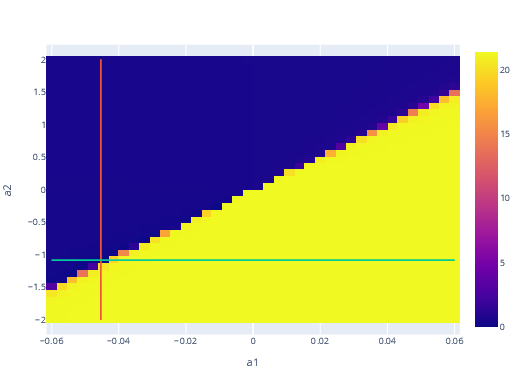
\includegraphics[scale=0.7]{imgs/c4/heat-1-entire.png}
    \caption{Objective value heatmap for fixed $\alpha$, with varying 
    $a_1$ and $a_2$}
    \label{heat-1-entire}
\end{figure}

\begin{figure}[h!]
    \centering
    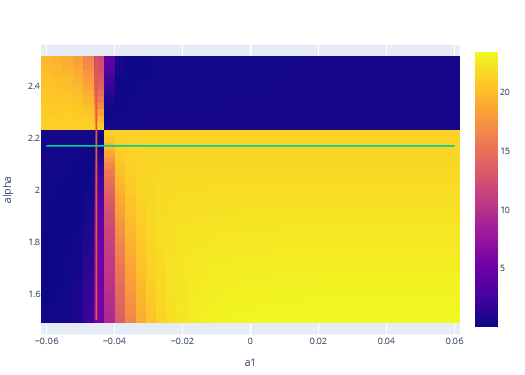
\includegraphics[scale=0.7]{imgs/c4/heat-2-entire.png}
    \caption{Objective value heatmap for fixed $a_2$, with varying 
    $a_1$ and $\alpha$}
    \label{heat-2-entire}
\end{figure}

\begin{figure}[h!]
    \centering
    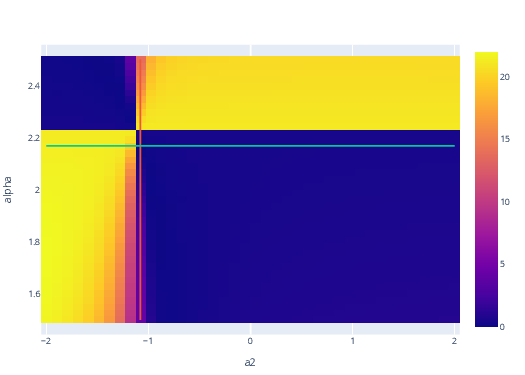
\includegraphics[scale=0.7]{imgs/c4/heat-3-entire.png}
    \caption{Objective value heatmap for fixed $a_1$, with varying 
    $a_2$ and $\alpha$}
    \label{heat-3-entire}
\end{figure}\newpage
The lines here point to the expected $(a_1, a_2, \alpha)$ values, and for each one 
we fix the parameter not being varied to be its expected value. Nevertheless, as we can see, our 
parameter space is quite binary, in that the distinction between suitable parameters and not is quite sharp, 
but with plateau's on either side - a nightmare situation for optimisation algorithms. If we zoom in 
around our expected parameters we indeed see even more strongly the sensitivity of our objective value to fluctuations in 
input parameters - see figures \ref{heat-1-zoomed} to \ref{heat-3-zoomed} in Appendix A.

Some of this behaviour is the result of the $(\alpha^2 - \lambda_{n,l}^2)^{-1}$ term introduced 
by $\psi$ in our objective function - it is this which motivates our usage of the MMA optimisation 
algorithm over more traditional methods like gradient descent, as we discussed in the previous section. 
However, as it stands - as an unconstrained optimisation problem - this is clearly still insufficient. 
One initial thought might be that our problem is simply underdetermined, and that by introducing more 
data we may improve the ability of our model to converge. However, as we see in figures \ref{heat-1-both} to \ref{heat-3-both},
the inclusion of pressure density profile data in our fitting attempts does not vastly improve our parameter space.

As such, the inclusion of extra data does not seem promising in our efforts to find a suitable set of parameters. Instead, 
our next effort was to constraint our problem - given we know what to expect our $P = (a_1, a_2, \alpha)$ values 
to be, we can constrain our parameter space by specifying a small offset for each. For example, 
if we know our parameter set is supposed to be $P' = (a_1', a_2', \alpha')$, then we can set
$$\Omega = [a_1' - \epsilon_{a_1}, a_1' + \epsilon_{a_1}] \times [a_2' - \epsilon_{a_2}, a_2' + \epsilon_{a_2}] \times [\alpha' - \epsilon_{\alpha}, \alpha' + \epsilon_{\alpha}]$$
For our intial parameter guess $P_0$ we can pick some random element of $\Omega$. When we introduce these constraints 
and turn our problem into a constrained optimisation problem we see significantly improved 
results, and our model converges - see figure \ref{solved-fig-1} as a recreation of figure 1 from Wang 
using simulateed current density profile data.

\begin{figure}[h!]
    \centering
    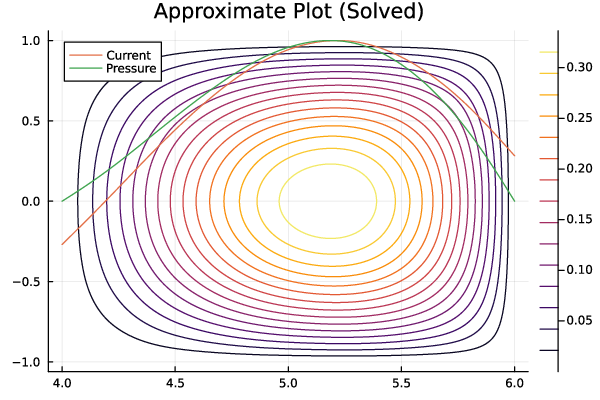
\includegraphics[scale=0.8]{imgs/c4/solved-fig-1.png}
    \caption{Equilibrium solution for the parameter set $P$ that we determine via optimisation, starting with a 
    set of current density profile data. This matches the expected figure 1 from Wang \cite{wang-analytic-solution}.}
    \label{solved-fig-1}
\end{figure}

\begin{figure}[h!]
    \centering
    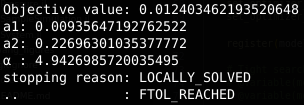
\includegraphics[scale=1]{imgs/c4/converged.png}
    \caption{Text output of our code showing convergence of our model.}
\end{figure}

Now that we can, for a given set of data, accurately derive the associated equilibrium solution, 
our next goal is simulate a current inversion given said data.

% 4.3
\section{Simulated Current Reversals}

We have the ability to solve for $P = (a_1, a_2, \alpha)$, and so now we will draw upon our 
work in chapter \ref{chapter3} in perturbing our equilibrium solution to simulate the effects of 
a time evolution, and in doing so, will observe how the system reacts.


% 4.3.1
\subsection{Method of Reversal}


\red{Linearly vary current. Could talk about alternatives - i.e. if 
our time perturbation had not been linear but had been trigonometric (to 
fit with a larger scope AC simulation) then our current reversal method 
here could be different}

\red{Feed solved parameters into guess for next. Emphasise problem of not knowing 
the initial ones nonetheless}


% 4.3.2
\subsection{Results and Explanations}

\red{Have still frame shots of the result of that (3x3 tiles?)}

\red{Show the slow version, then the 'zoomed' in version}

\red{Highlight magnetic field topology breaking - suggests RE population generation}

\red{Comment on feasibility of the behaviour - e.g.pressure density profile follows 
magnetic field axis, but then there are things like current densities 
at the edge of the reactor}

